%%%%%%%%%%%%%%%%%%%%%%%%%%%%%%%%%%%%%%%%%%%%%%%%%%%%%%%%%%%%%%%%%%%%%
% LaTeX Template: Project Titlepage Modified (v 0.1) by rcx
%
% Original Source: http://www.howtotex.com
% Date: February 2014
% 
% This is a title page template which be used for articles & reports.
% 
% This is the modified version of the original Latex template from
% aforementioned website.
% 
%%%%%%%%%%%%%%%%%%%%%%%%%%%%%%%%%%%%%%%%%%%%%%%%%%%%%%%%%%%%%%%%%%%%%%
\documentclass[openany,11pt]{report}%report
\usepackage[a4paper]{geometry}
\usepackage[myheadings]{fullpage}
\usepackage{fancyhdr}
\usepackage{fancybox}	
\usepackage{lastpage}
\usepackage{color}
\usepackage{graphicx}
\usepackage{wrapfig, subcaption, setspace, booktabs}
\usepackage[T1]{fontenc}
\usepackage[font=small, labelfont=bf]{caption}
\usepackage{fourier}
\usepackage[protrusion=true, expansion=true]{microtype}
\usepackage[english]{babel}
\usepackage{sectsty}
\usepackage{url, lipsum}
\usepackage{mathtools}
\usepackage{makeidx}
\usepackage{float}
\newcommand{\HRule}[1]{\rule{\linewidth}{#1}}
\onehalfspacing
\widowpenalty = 10000
\clubpenalty = 10000
\usepackage{pdflscape}
\usepackage{tikz-cd}
\usepackage{tikz}
\usetikzlibrary{shapes,arrows,calc,trees,positioning}
\usetikzlibrary{chains,fit,shapes.geometric,shapes.arrows}
\usepackage{forest}
\usetikzlibrary{arrows.meta, shapes.geometric, calc, shadows}
\usetikzlibrary{arrows,automata}
\usetikzlibrary{trees}
\usetikzlibrary{decorations.text}
\usetikzlibrary{shapes.geometric,arrows.meta,decorations.markings}
\usepackage{pgfgantt}
\usetikzlibrary{mindmap}
\usepackage{subcaption}
\usepackage{csquotes}
\usepackage{amsmath}
\usepackage{tabularx}
\usepackage{tabulary}
\usepackage{booktabs}
\usepackage{siunitx}
\usepackage{booktabs}
\usepackage{colortbl}
\usetikzlibrary{calc}
\usepackage{smartdiagram}
\usepackage{wrapfig}
\usesmartdiagramlibrary{additions}	
\usepackage{multirow}
\usepackage{subcaption}
\usepackage{makecell}
\usepackage{forest}
\usepackage{here}
\usepackage{url} 
\usepackage{csquotes}
\usepackage{afterpage}
\usepackage{xcolor}
\usepackage{longtable}
\usepackage{comment}
\usepackage{listings}
\usepackage{fancyvrb}
\usepackage{wasysym}
\usepackage{adjustbox,lipsum}
\usepackage{amssymb}
\usepackage{makecell}
\usepackage{bigints}
%\usepackage{ascmac}
\usepackage{cancel}
\usepackage{hyperref}

%Makecell, used to add linebreak to tables
\renewcommand\theadalign{bc}
\renewcommand\theadfont{\bfseries}
\renewcommand\theadgape{\Gape[4pt]}
\renewcommand\cellgape{\Gape[4pt]}

%-------------------------------------------------------------------------------
% CODE  Style
%-------------------------------------------------------------------------------

%\definecolor{mauve}{rgb}{0.87, 0.69, 0.8}
%\definecolor{dkgreen}{rgb}{0.0, 0.2, 0.13}

\lstdefinestyle{DOS}
{
    backgroundcolor=\color{black},
    basicstyle=\small\color{white}\ttfamily
}

\lstdefinestyle{INI}{% define own style
  basicstyle=\ttfamily\small,
    columns=fullflexible,
    morecomment=[s][\color{blue}\bfseries]{[}{]},
    morecomment=[l]{\#},
    morecomment=[l]{;},
    commentstyle=\color{gray}\ttfamily,
    morekeywords={},
    otherkeywords={=,:},
      frame=single,                   % adds a frame around the code
    keywordstyle={\color{black}\bfseries}
}

\lstdefinelanguage{json}{
    basicstyle=\ttfamily\small,
    numbers=left,
    numberstyle=\scriptsize,
    stepnumber=1,
    numbersep=8pt,
    showstringspaces=false,
    breaklines=true,
    frame=lines,
    backgroundcolor=\color{background},
    literate=
     *{0}{{{\color{numb}0}}}{1}
      {1}{{{\color{numb}1}}}{1}
      {2}{{{\color{numb}2}}}{1}
      {3}{{{\color{numb}3}}}{1}
      {4}{{{\color{numb}4}}}{1}
      {5}{{{\color{numb}5}}}{1}
      {6}{{{\color{numb}6}}}{1}
      {7}{{{\color{numb}7}}}{1}
      {8}{{{\color{numb}8}}}{1}
      {9}{{{\color{numb}9}}}{1}
      {:}{{{\color{punct}{:}}}}{1}
      {,}{{{\color{punct}{,}}}}{1}
      {\{}{{{\color{delim}{\{}}}}{1}
      {\}}{{{\color{delim}{\}}}}}{1}
      {[}{{{\color{delim}{[}}}}{1}
      {]}{{{\color{delim}{]}}}}{1},
}

%-------------------------------------------------------------------------------
% HEADER & FOOTER
%-------------------------------------------------------------------------------
\pagestyle{fancy}
\fancyhf{}
\setlength\headheight{15pt}
\fancyhead[L]{GAIL User Manual}
\fancyhead[R]{TDI-202006-JQ0081}
\setcounter{secnumdepth}{4}

%-------------------------------------------------------------------------------
% Table of Content / Index
%-------------------------------------------------------------------------------
\makeindex
%-------------------------------------------------------------------------------
% Extra
%-------------------------------------------------------------------------------

%%Changing chapter name with section
%\makeatletter
%\renewcommand{\@chapapp}{Section}
%\makeatother

\def\changemargin#1#2{\list{}{\rightmargin#2\leftmargin#1}\item[]}
\let\endchangemargin=\endlist 

%running fraction with slash - requires math mode.
\newcommand*\rfrac[2]{{}^{#1}\!/_{#2}}

%Bit larger cells for arrays
\renewcommand{\arraystretch}{1.5}


\tikzset{description title/.append style={
    signal, 
   signal to=south, 
    signal from=north,
    minimum width=2.0cm,
    yshift=-0.2cm,
  }
}
\newcommand{\bm}[1]{{\mbox{\boldmath $#1$}}}

\date{
    \normalsize{June 22, 2020}
    }

%-------------------------------------------------------------------------------
% TITLE PAGE
%-------------------------------------------------------------------------------

\begin{document}

\title{ \HRule{0.5pt} \\
		\LARGE \textbf{\uppercase{GAIL}}\\
	    \textbf{\sc{User Manual}}\\
		\HRule{2pt} \\ [0.5cm]
		\normalsize  \vspace*{8\baselineskip}
		}

\maketitle

\newpage


\textit{Revision History}
\vspace*{0.2in} 	 

\begin{tabular}{|c||c|p{10cm}|}
\hline 
Version & Date & Modification \\ 
\hline 
\hline 
1.00& 10/JUNE/2020 & Draft.\\\hline
1.10& 22/JUNE/2020 & Final release.\\\hline
\end{tabular} 

\newpage
\tableofcontents
\clearpage

\pagestyle{plain}

\chapter{Overview}
In this document, the items included in the GAIL package for Generative Adversarial Imitation Learning are described. In addition, the dependency information, the compilation procedure and the execution procedure of the application are provided.

\chapter{Package Structure}

\definecolor{folderbg}{RGB}{124,166,198}
\definecolor{folderborder}{RGB}{110,144,169}

\def\Size{4pt}
\tikzset{
  folder/.pic={
    \filldraw[draw=folderborder,top color=folderbg!50,bottom color=folderbg]
      (-1.05*\Size,0.2\Size+5pt) rectangle ++(.75*\Size,-0.2\Size-5pt);  
    \filldraw[draw=folderborder,top color=folderbg!50,bottom color=folderbg]
      (-1.15*\Size,-\Size) rectangle (1.15*\Size,\Size);
  }
}

\tikzset{
  file/.pic={
    \filldraw [draw=folderborder, top color=folderbg!5, bottom color=folderbg!10]
    (-\Size,.4*\Size+3pt) coordinate (a) |- (\Size,-1.2*\Size) coordinate (b) -- ++(0,1.6*\Size)
    coordinate (c) -- ++(-3pt,3pt) coordinate (d) -- cycle (d) |- (c) ;
  }
}

\begin{figure}[H]
\begin{forest}
  for tree={
    font=\ttfamily,
    grow'=0,
    child anchor=west,
    parent anchor=south,
    anchor=west,
    calign=first,
    inner xsep=7pt,
    edge path={
      \noexpand\path [draw, \forestoption{edge}]
      (!u.south west) +(7.5pt,0) |- (.child anchor) pic {folder} \forestoption{edge label};
    },
    file/.style={edge path={\noexpand\path [draw, \forestoption{edge}]
          (!u.south west) +(7.5pt,0) |- (.child anchor) pic {file} \forestoption{edge label};}
    },
    before typesetting nodes={
      if n=1
        {insert before={[,phantom]}}
        {}
    },
    fit=band,
    before computing xy={l=15pt},
  }
[Package root
[{\bf gail-driver} : GAIL training inference tool.
]
[{\bf AutomotiveDrivingModels} : automobile simulator.
]
[{\bf AutoVis} : automobile simulator visualizer.
]
[{\bf NGSIM} : next generation automobile simulator 
]
[{\bf ForwardNets.jl} : External libraries.
]
[{\bf Records.jl} : 
]
]
\end{forest}
  \caption{folder structure}
  \label{fig:folder_struct}
\end{figure}

\chapter{Installation}
Requirements: Computer running Ubuntu 18.04 (x86\_64(Intel)). Compiler: g$++$ version 7.  JULIA 0.6.4, Python 2.7, Anaconda2 version 5.3.0.

\textbf{Note: Please check the compiler (g$++$) version before all work. gcc/g$++$ version must be 7.}

\section{Installing g$++$ version 7}

The code needs g++ version 7 or superior to compile. To check the compiler version:
\begin{lstlisting}[style=DOS]
xterm:\> g++ -v
\end{lstlisting}

If it is 7 or above, no update is needed. You may proceed to the download and installation of Eclipse. If not, install gcc/c++ version 7:

\begin{lstlisting}[style=DOS]
xterm:\> sudo apt update
xterm:\> sudo apt upgrade
xterm:\> sudo apt install gcc
xterm:\> sudo apt install g++
xterm:\> sudo apt install hdf5-tools
\end{lstlisting}

Register different versions:
\begin{lstlisting}[style=DOS]
xterm:\> sudo sh register.sh
\end{lstlisting}
The file register.sh is attached in the package root folder. Next: set g++ 7 as default:

\begin{lstlisting}[style=DOS]
xterm:\> sudo update-alternatives --config gcc
  Selection    Path            Priority   Status
------------------------------------------------------------
* 0            /usr/bin/gcc-7   70        auto mode
  1            /usr/bin/gcc-5   50        manual mode
  2            /usr/bin/gcc-7   70        manual mode

Press <enter> to keep the current choice[*], or type selection number:
\end{lstlisting}
Press 0 and return. Confirm the default version.
\begin{lstlisting}[style=DOS]
xterm:\> g++ -v
\end{lstlisting}


%これから作る環境は以下の構造を想定している。

\begin{figure}[H]
\begin{forest}
  for tree={
    font=\ttfamily,
    grow'=0,
    child anchor=west,
    parent anchor=south,
    anchor=west,
    calign=first,
    inner xsep=7pt,
    edge path={
      \noexpand\path [draw, \forestoption{edge}]
      (!u.south west) +(7.5pt,0) |- (.child anchor) pic {folder} \forestoption{edge label};
    },
    file/.style={edge path={\noexpand\path [draw, \forestoption{edge}]
          (!u.south west) +(7.5pt,0) |- (.child anchor) pic {file} \forestoption{edge label};}
    },
    before typesetting nodes={
      if n=1
        {insert before={[,phantom]}}
        {}
    },
    fit=band,
    before computing xy={l=15pt},
  }
[Package root
[{\bf gail} : GAIL directory
 [{\bf gail-driver} : GAIL driver directory
 ]
]
[{\bf julia} : Julia environment directory
 [{\bf julia-0.6.4} : Julia compiler/interpreter directory
 ]
]
[{\bf .julia} : Julia programs directory
]
[{\bf anaconda2} : Anaconda2 and python directory
]
]
\end{forest}
  \caption{folder structure}
  \label{fig:folder_struct}
\end{figure}


\begin{lstlisting}[style=DOS]
xterm:\> mkdir julia
xterm:\> mkdir gail
\end{lstlisting}


\section{Install Anaconda2 5.3}

Getting Anaconda2 installer.

\begin{lstlisting}[style=DOS]
xterm:\> wget https://repo.anaconda.com/archive/
 Anaconda2-5.3.0-Linux-x86_64.sh
xterm:\> chmod +x ./Anaconda2-5.3.0-Linux-x86_64.sh
xterm:\> ./Anaconda2-5.3.0-Linux-x86_64.sh
xterm:\> source ./.bashrc
\end{lstlisting}


\begin{lstlisting}[style=DOS]
xterm:\> python
\end{lstlisting}

\begin{figure}[h]
    \centering
    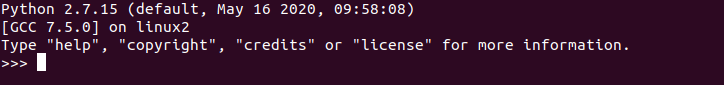
\includegraphics[width=\textwidth]{img/python.png}
    \label{fig: python versin}
\end{figure}

\section{Install Julia version 0.6}
Requirements: Julia version 0.6 fix.  (0.5, 0.7 are both incompatible as 0.6j)

It is needed to refresh/upgrade the pre-installed packages/libraries:
\begin{lstlisting}[style=DOS]
xterm:\> cd julia 
xterm:\> wget https://julialang-s3.julialang.org/bin/linux/x64/0.6/
 julia-0.6.4-linux-x86_64.tar.gz
xterm:\> tar xzvf julia-0.6.4-linux-x86_64.tar.gz
xterm:\> mv julia-9d11f62bcb julia-0.6.4
xterm:\> sudo ln -s /home/[username]/julia/julia-0.6.4/bin/julia \
 /usr/local/bin/julia
xterm:\> cd ..
\end{lstlisting}

%チェックのため、 JULIA とタイプすると、JULIA 環境になる。

\begin{lstlisting}[style=DOS]
xterm:\> julia
\end{lstlisting}

\begin{figure}[h]
    \centering
    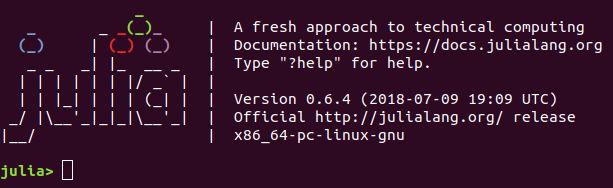
\includegraphics[width=\textwidth]{img/julia.png}
    \label{fig: 2DMOT2015}
\end{figure}



\section{Install packages NGSIM/AutomoticeDrivingModels/ForwardNets}



\begin{lstlisting}[style=DOS]
xterm:\> cd gail    #-> ~/gail
xterm:\> git clone https://github.com/[install_url]/gail-driver
xterm:\> export GAIL_DRIVER_GITHUB="https://github.com/[install_url]/"
xterm:\> cd gail-driver
xterm:\> julia julia_package_install.jl
xterm:\> chmod +x python_package_install.sh
xterm:\> ./python_package_install.sh
xterm:\> cd ../..
\end{lstlisting}


To connect python and julia.

\begin{lstlisting}[style=DOS]
xterm:\> julia
\end{lstlisting}
\begin{lstlisting}[style=DOS]
julia> Pkg.init()
julia> Pkg.add("PyCall") 
julia> using PyCall
julia> ENV["PYTHON"]="/home/[username]/anaconda2/bin/python"
julia> rm(Pkg.dir("PyCall","deps","PYTHON"))
julia> Pkg.build("PyCall")
julia> exit() # escape from JULIA terminal 
\end{lstlisting}

On ubuntu terminal.
\begin{lstlisting}[style=DOS]
xterm:\> export CONDA_JL_HOME="/home/[username]/anaconda2/bin"
xterm:\> sudo julia -e 'Pkg.build("Conda")'
\end{lstlisting}

On julia terminal.
\begin{lstlisting}[style=DOS]
julia> Pkg.add("IJulia")
julia> Pkg.add("PyPlot")
julia> Pkg.update()
\end{lstlisting}

On python terminal.
\begin{lstlisting}[style=DOS]
python> import julia
python> julia.install()
\end{lstlisting}



\section{Install gail-driver}


\begin{lstlisting}[style=DOS]
xterm:\> export PYTHONPATH="/home/[userinstall]/gail/gail-driver:PYTHONPATH"
\end{lstlisting}
%(これは、.bashrc にも記載するとよい)

Make directory. "~/gail/gail-driver/data".

\begin{figure}[H]
\begin{forest}
  for tree={
    font=\ttfamily,
    grow'=0,
    child anchor=west,
    parent anchor=south,
    anchor=west,
    calign=first,
    inner xsep=7pt,
    edge path={
      \noexpand\path [draw, \forestoption{edge}]
      (!u.south west) +(7.5pt,0) |- (.child anchor) pic {folder} \forestoption{edge label};
    },
    file/.style={edge path={\noexpand\path [draw, \forestoption{edge}]
          (!u.south west) +(7.5pt,0) |- (.child anchor) pic {file} \forestoption{edge label};}
    },
    before typesetting nodes={
      if n=1
        {insert before={[,phantom]}}
        {}
    },
    fit=band,
    before computing xy={l=15pt},
  }
[Package root
[{\bf gail} : GAIL directory
 [{\bf gail-driver} : GAIL driver directory
  [{\bf data} :
   [\textcolor{red}{NGSIM\_train\_test\_split.h5}]
   [\textcolor{red}{core1\_temp0\_well1\_neig0\_carl1 .... \_clmr100\_rlmr50\_seed456.h5}
   ]
  ]
  [{\bf julia} 
   [{\bf validation} 
    [{\bf models} 
     [\textcolor{red}{gail\_mlp.h5}]
     [\textcolor{red}{gail\_gru.h5}]
     [\textcolor{red}{bc\_mlp.h5}]
     [\textcolor{red}{bc\_gru.h5}]
    ]
    [\textcolor{red}{RootDir.jl}]
   ]
  ]
 ]
]
[{\bf .julia} : Julia package directory
 [{\bf v0.6} : version 0.6
  [{\bf NGSIM} 
   [{\bf data} :
    [\textcolor{red}{i80\_trajectories-0400-0415.txt}]
    [\textcolor{red}{i80\_trajectories-0500-0515.txt}]
    [\textcolor{red}{i80\_trajectories-0515-0530.txt}]
    [\textcolor{red}{i101\_trajectories-0750am-0415am.txt}]
    [\textcolor{red}{i101\_trajectories-0805am-0515am.txt}]
    [\textcolor{red}{i101\_trajectories-0820am-0530am.txt}]
    [\textcolor{red}{trajdata\_i80\_trajectories-0400-0415.txt}]
    [\textcolor{red}{trajdata\_i80\_trajectories-0500-0515.txt}]
    [\textcolor{red}{trajdata\_i80\_trajectories-0515-0530.txt}]
    [\textcolor{red}{trajdata\_i101\_trajectories-0750am-0415am.txt}]
    [\textcolor{red}{trajdata\_i101\_trajectories-0805am-0515am.txt}]
    [\textcolor{red}{trajdata\_i101\_trajectories-0820am-0530am.txt}]
   ]
  ]
 ]
]
]
\end{forest}
  \caption{folder structure}
  \label{fig:folder_struct}
\end{figure}
\begin{lstlisting}[style=DOS]
xterm:\> import julia
\end{lstlisting}

The file RootDir.jl must be made.
\begin{lstlisting}[style=DOS]
ROOT_FILEPATH="/home/[username]/gail/gail-driver/"
\end{lstlisting}

Now on writting ...

JULIA modules are premised on github.
Here will show how to register to github and download from githib.


\chapter{Data for experiments}

For all data used in the experiment, include the address of website.

(The acquired data will be included in the package.)


Now on writting.......

\section{Generating Filtered Trajectory}

Filtered trajectories are also necessary for experiment.

(The generated trajectories will be included in the package.)

Following trajectory data must be generate by using observed data and NGSIM library.
This section describes how to generate the filtered data. 

\begin{itemize}
\item trajdata\_i80\_trajectories-0400-0415.txt
\item trajdata\_i80\_trajectories-0500-0515.txt
\item trajdata\_i80\_trajectories-0515-0530.txt
\item trajdata\_i101\_trajectories-0750am-0415am.txt
\item trajdata\_i101\_trajectories-0805am-0515am.txt
\item trajdata\_i101\_trajectories-0820am-0530am.txt
\end{itemize}


\chapter{Introduction of external modules for experiments}

Now writing ...


Julia and python important modules.

\begin{itemize}
\item AutomotiveDrivingModels.jl
\item NGSIM.jl
\item AutoViz.jl
\item ForwardNets.jl
\item rllab
\item AutoDrivers.jl
\end{itemize}

writing about ...

\begin{itemize}
\item address on github
\item commit id
\item tag, branch, and other information.
\item summary of each module.
\end{itemize}



\end{document}

